\documentclass[conference]{IEEEtran}
\usepackage{cite,graphicx,booktabs,url,tabularx}
\begin{document}
\title{rf-frontend: Design, Verification and Release Evidence for Hardware Revision A}
\author{\IEEEauthorblockN{Author Name}\IEEEauthorblockA{Affiliation\\email@example.com}}
\maketitle
\begin{abstract}
% Auto-generated skeleton. Replace with the actual contribution statement.
This paper documents the requirements, design method, verification and release evidence of a pcb-scope electronic product.
The design was developed with an iterative modify--verify--retain loop (11 retained of 13 candidate changes) and gated by
electrical-rule, design-rule, corner simulation and rule-based checks. The current gate result is \texttt{G3\_BLOCKED}.
\end{abstract}
\begin{IEEEkeywords}
hardware design, verification, PCB, design rules, evidence
\end{IEEEkeywords}

\section{Introduction}
State the problem, intended use and the contribution. Sources consulted during design: \cite{archambeault2002} \cite{bogatin2018} \cite{bowick2008} \cite{brooks2021} \cite{horowitz2015} \cite{johnson2003} \cite{paul2022} \cite{williams2016} \cite{wilson2011}.

\section{Requirements}
\begin{table*}[!t]
\caption{Requirements baseline}
\label{tab:reqs}
\centering
\scriptsize
\begin{tabularx}{\textwidth}{l|>{\raggedright\arraybackslash}X|l|>{\raggedright\arraybackslash}X|l|l}
\hline
\textbf{id} & \textbf{statement} & \textbf{units} & \textbf{conditions} & \textbf{method} & \textbf{gate} \\
\hline
HR-001 & RF input and output networks: return loss $\ge$ 15 dB and insertion loss $\le$ 0.6 dB from 2.3 to 2.5 GHz (connector landing to gain-block pin) & dB & full-wave model of the released copper, 50 ohm ports & simulation & G3 \\
HR-002 & Every RF line 50 ohm +/-10 \% on the fabricator stackup & ohm & field solution of the routed cross-section incl. mask and coplanar gaps & analysis & G3 \\
HR-003 & Gain-block bias current 100 mA +/-10 \% from the 12 V input (device voltage 4.4 V typ, datasheet value to confirm) & mA & 12 V +/-10 \% input, 25 C & analysis & G3 \\
HR-004 & Every resistor at or below 50 \% of its rated power (2x derating) & \% & worst-case 13.2 V input, 70 C ambient rating & analysis & G3 \\
HR-005 & 25 MHz clock into a 50 ohm load: overshoot $\le$ 15 \%, ringback $\le$ 20 \%, settled within 5 ns & \% & routed clock net, 1 ns edges & simulation & G3 \\
HR-006 & +3V3 rail impedance at the oscillator below Z\_target (2 \% ripple on a 20 mA step) from 1 kHz to 100 MHz & ohm & released capacitor set and planes & analysis & G3 \\
HR-007 & Every dissipating part at least 20 C below its maximum junction/element temperature & C & 40 C still air, board horizontal & analysis & G3 \\
HR-008 & Clock-harmonic radiated-emission estimate at least 6 dB below CISPR 32 Class B (estimate only; chamber test at EVT) & dB & routed clock loops, 10 m limit line & analysis & G3 \\
HR-009 & 12 V input path: trace temperature rise $\le$ 10 C at 150 mA & C & IPC-2152 external/internal fits & analysis & G3 \\
HR-010 & Schematic connectivity equals the golden circuit description & nets & fresh KiCad netlist export & inspection & G3 \\
HR-011 & Assembled board: measured S11 $\le$ -10 dB from 2.3 to 2.5 GHz at both RF ports & dB & VNA, calibrated at the SMA reference planes & test & G4 \\
\hline
\end{tabularx}
\end{table*}


\section{Design Method}
Describe the architecture and the design rules applied (see Table~\ref{tab:decisions}).
\begin{table*}[!t]
\caption{Design decisions and the rules that justify them}
\label{tab:decisions}
\centering
\scriptsize
\begin{tabularx}{\textwidth}{l|l|>{\raggedright\arraybackslash}X|>{\raggedright\arraybackslash}X|>{\raggedright\arraybackslash}X}
\hline
\textbf{id} & \textbf{topic} & \textbf{decision} & \textbf{rules} & \textbf{sources} \\
\hline
D-1 & RF line & 0.32 mm grounded coplanar, 0.3 mm pour gap, 0.2 mm prepreg to In1 GND: 49.7 ohm & - & tools/size\_rf\_line.py field solver \\
D-2 & Bias & 12 V through 3 x 220R 2512 (73.3 ohm) + 22 nH choke; 104 mA & AOE-3330;WILSON-394 & design/rules.tsv R-01..R-03 \\
D-3 & Stackup & 4 layers: F.Cu RF over In1 GND, In2 +3V3 plane, B.Cu GND pour & BOGATIN-2147 & tools/make\_template.py \\
D-4 & Routing & RF, clock output, fences, stitching and plane fanouts pre-routed and locked; Freerouting for the rest & ARCH-065;WILLIAMS-2038 & tools/make\_routes.py \\
D-5 & Edge launch & SMA pads pulled back 0.3 mm; board floor 0.25 mm, 0.5 mm rule for everything else & - & pcb/rffe.kicad\_dru \\
D-6 & RF rule frequency & fence/stitching judged at 5 GHz (2nd harmonic of the 2.5 GHz band edge) & ARCH-065;WILLIAMS-2038 & design/rf.tsv \\
D-7 & Track floor & board minimum track 0.15 mm (fab capability); Freerouting necks the bias line to 0.15 mm at pins & BROOKS-046 & layout check: BIAS IPC-2152 rise on the narrowest segment \\
D-8 & SMA launch & In1 and In2 cut out under the J1/J2 centre pads (1.0 mm beyond each side): the 1.5 mm pad references B.Cu, 47.8 ohm field-solved & JOHNSON03-1307;JOHNSON03-1278 & johnson2003; openEMS rf\_in; tools/make\_template.py \\
D-9 & DC blocks and RF bypass & C1/C2/C3 10 pF C0G 0402: series-resonant near the band with the body ESL, \textbar{}X\textbar{} $\le$ 3.1 ohm from 2.3 to 2.5 GHz & BOGATIN-167;BOGATIN-2128;ARCH-067;AOE-3330 & design/rules.tsv R-05/R-06/R-11 \\
\hline
\end{tabularx}
\end{table*}


\section{Verification}
Every check executed is recorded as a hashed receipt (Table~\ref{tab:exec}); the closest call of each, relative to its limit, is in Table~\ref{tab:margins}.
\begin{table*}[!t]
\caption{Execution instances}
\label{tab:exec}
\centering
\scriptsize
\begin{tabularx}{\textwidth}{l|l|l|>{\raggedright\arraybackslash}X|l}
\hline
\textbf{check} & \textbf{status} & \textbf{method} & \textbf{tool} & \textbf{created} \\
\hline
AUTO-CONNECTIVITY & pass & inspection & 10.0.5 & 2026-10-01T05:36:14.688618+00:00 \\
AUTO-DRC & pass & inspection & 10.0.5 & 2026-10-01T05:36:12.040523+00:00 \\
AUTO-EMC & pass & analysis & python 3.13.7; kicad-cli 10.0.5 & 2026-10-01T05:37:44.894011+00:00 \\
AUTO-ERC & pass & inspection & 10.0.5 & 2026-10-01T05:36:09.915209+00:00 \\
AUTO-LAYOUT & pass & analysis & python 3.13.7; kicad-cli 10.0.5 & 2026-10-01T05:36:45.496021+00:00 \\
AUTO-PDN & pass & analysis & python 3.13.7; kicad-cli 10.0.5 & 2026-10-01T05:37:29.648165+00:00 \\
AUTO-RULES & pass & analysis & 3.13.7 & 2026-10-01T05:36:14.969774+00:00 \\
AUTO-SI & pass & simulation & python 3.13.7; kicad-cli 10.0.5; ngspice-47 : Circuit level simulation program & 2026-10-01T05:37:34.090480+00:00 \\
AUTO-SIM & pass & simulation & ngspice-47 : Circuit level simulation program & 2026-10-01T05:36:13.721656+00:00 \\
AUTO-THERMAL & pass & analysis & python 3.13.7; kicad-cli 10.0.5 & 2026-10-01T05:37:38.303300+00:00 \\
\hline
\end{tabularx}
\end{table*}

\begin{table*}[!t]
\caption{Closest call of each check, relative to its limit (every row: AUDIT.md)}
\label{tab:margins}
\centering
\scriptsize
\begin{tabularx}{\textwidth}{l|>{\raggedright\arraybackslash}X|>{\raggedright\arraybackslash}X|l|l|l|l}
\hline
\textbf{check} & \textbf{id} & \textbf{corner} & \textbf{value} & \textbf{units} & \textbf{margin} & \textbf{status} \\
\hline
AUTO-EMC & CLK\_OUT:excess\_over\_cispr32\_b &  & -32.2248 & dB & 26.2248313 & PASS \\
AUTO-LAYOUT & /RF\_B:z0@F.Cu/0.32mm &  & 51.4157 & ohm & 3.5842539 & PASS \\
AUTO-PDN & +3V3:z\_pdn\_max &  & 0.803463 & ohm & 0.846537216 & PASS \\
AUTO-RULES & R-01 &  & 103.641 & mA & 6.358925 & PASS \\
AUTO-SI & /CLK\_OUT@J3.1:ringback &  & 9.75582 & \% & 10.2441787 & PASS \\
AUTO-SIM & S-2 & \{"ctol": "0.8", "rd": "20", "rtol": "0.95"\} & -3.09513e+01 & dB & 20.9513 & PASS \\
AUTO-THERMAL & U2:tj &  & 129.031 & C & 0.968688 & PASS \\
\hline
\end{tabularx}
\end{table*}

\begin{figure}[!t]
\centering
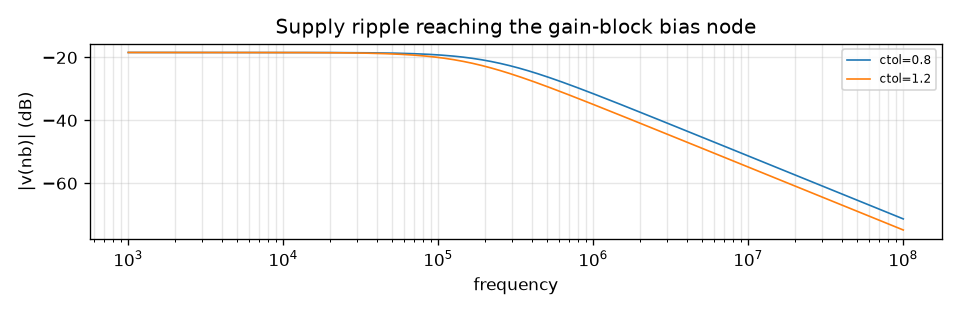
\includegraphics[width=\columnwidth,height=0.45\textheight,keepaspectratio]{../../audit/plots/P-1.png}
\caption{Circuit simulation at declared corners: P-1}
\label{fig:plots-P-1}
\end{figure}
\begin{figure}[!t]
\centering
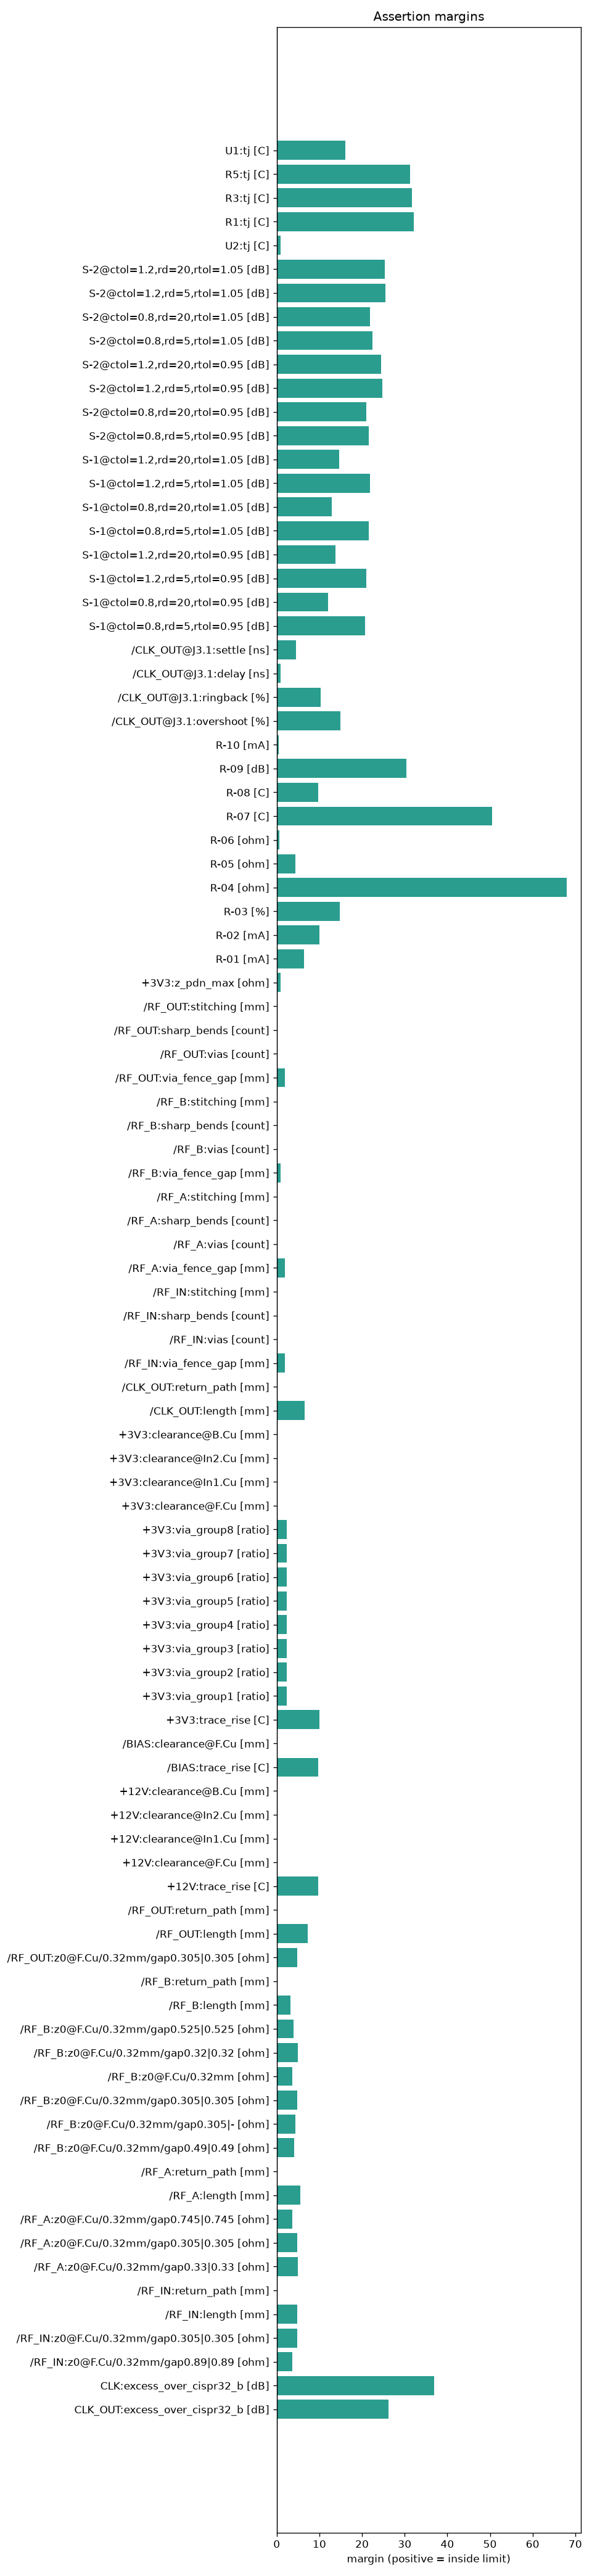
\includegraphics[width=\columnwidth,height=0.45\textheight,keepaspectratio]{../../audit/plots/margins.png}
\caption{Assertion margins of every check: margins}
\label{fig:plots-margins}
\end{figure}
\begin{figure}[!t]
\centering
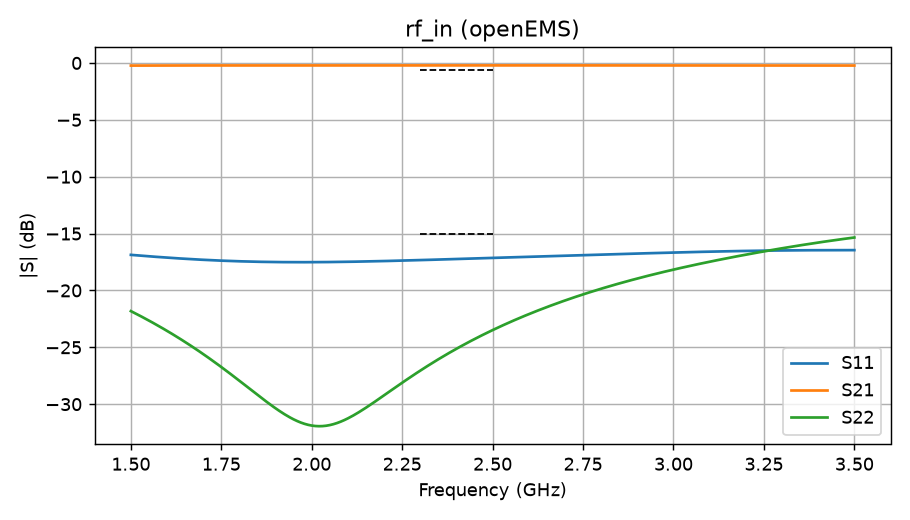
\includegraphics[width=\columnwidth,height=0.45\textheight,keepaspectratio]{../../analysis/em/rf_in.png}
\caption{openEMS S-parameters of the board copper: rf\_in}
\label{fig:em-rf-in}
\end{figure}
\begin{figure}[!t]
\centering
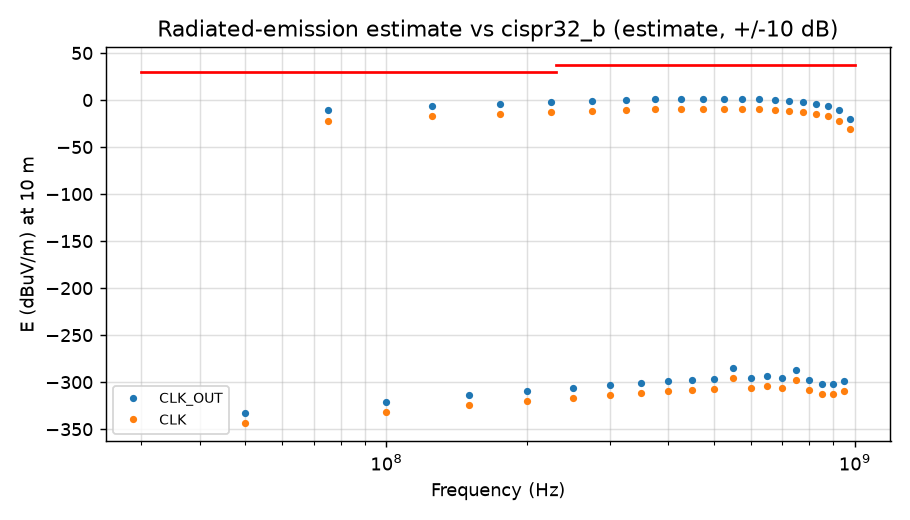
\includegraphics[width=\columnwidth,height=0.45\textheight,keepaspectratio]{../../analysis/emc/emc-cispr32_b.png}
\caption{Radiated-emission estimate against the limit line: emc-cispr32\_b}
\label{fig:emc-emc-cispr32-b}
\end{figure}
\begin{figure}[!t]
\centering
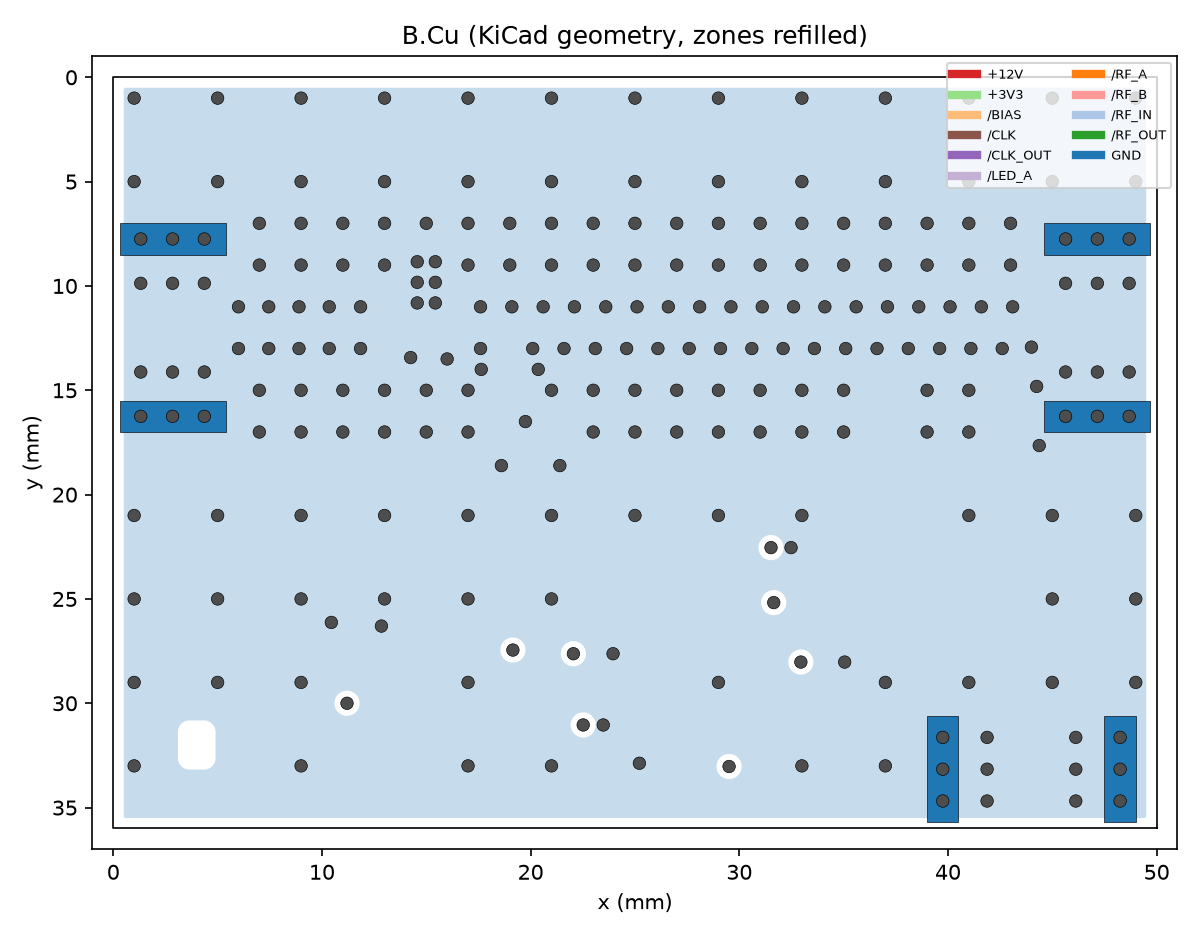
\includegraphics[width=\columnwidth,height=0.45\textheight,keepaspectratio]{../../analysis/layout/copper-B_Cu.png}
\caption{Copper: copper-B\_Cu}
\label{fig:layout-copper-B-Cu}
\end{figure}
\begin{figure}[!t]
\centering
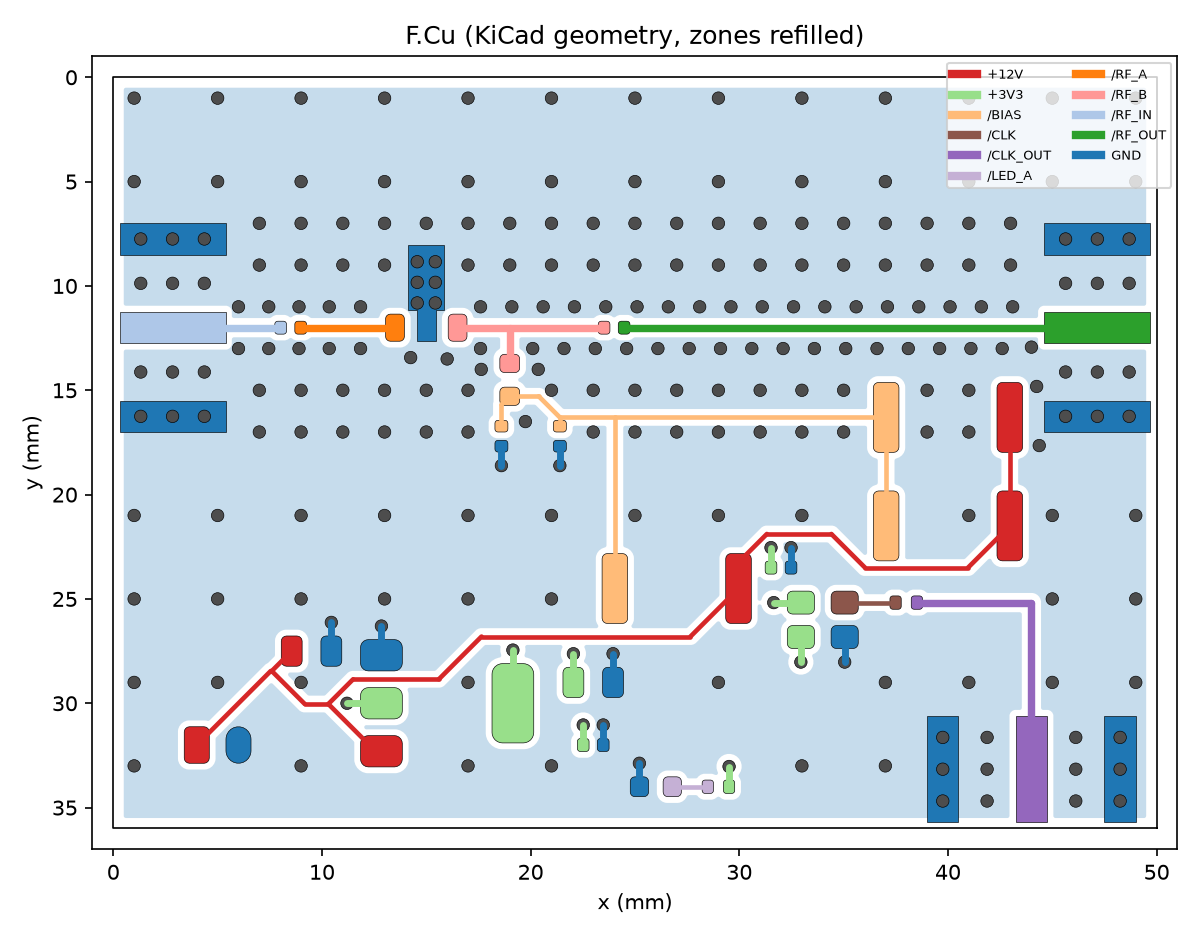
\includegraphics[width=\columnwidth,height=0.45\textheight,keepaspectratio]{../../analysis/layout/copper-F_Cu.png}
\caption{Copper: copper-F\_Cu}
\label{fig:layout-copper-F-Cu}
\end{figure}
\begin{figure}[!t]
\centering
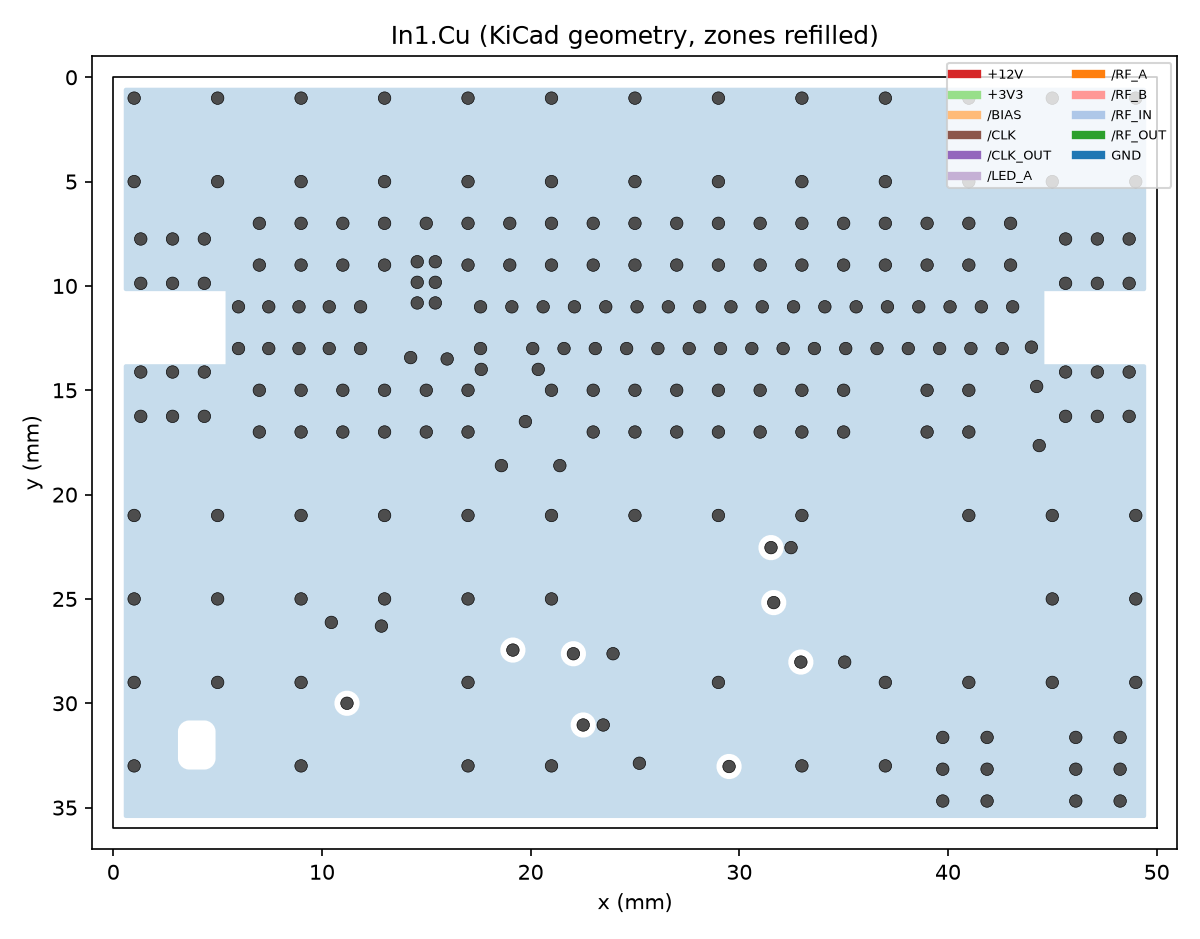
\includegraphics[width=\columnwidth,height=0.45\textheight,keepaspectratio]{../../analysis/layout/copper-In1_Cu.png}
\caption{Copper: copper-In1\_Cu}
\label{fig:layout-copper-In1-Cu}
\end{figure}
\begin{figure}[!t]
\centering
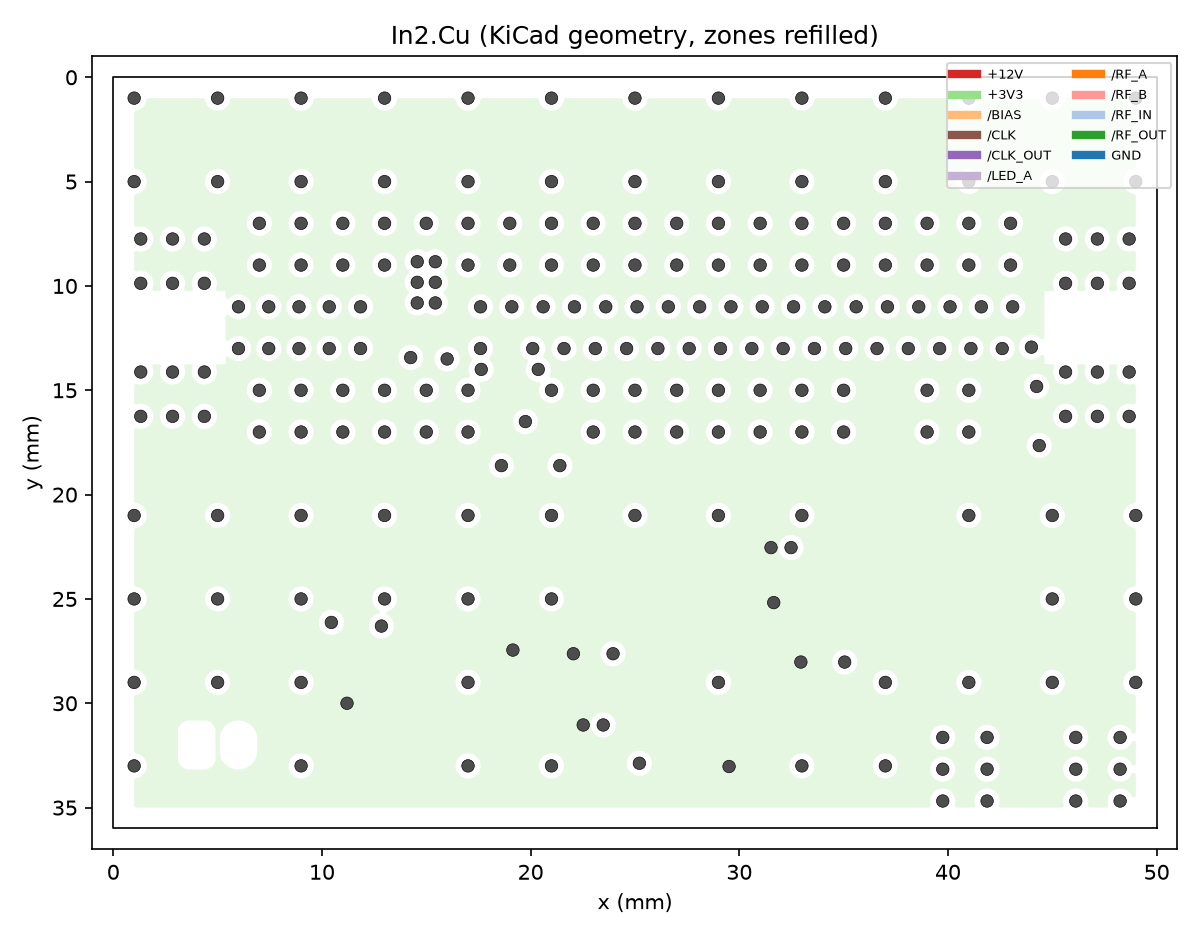
\includegraphics[width=\columnwidth,height=0.45\textheight,keepaspectratio]{../../analysis/layout/copper-In2_Cu.png}
\caption{Copper: copper-In2\_Cu}
\label{fig:layout-copper-In2-Cu}
\end{figure}
\begin{figure}[!t]
\centering
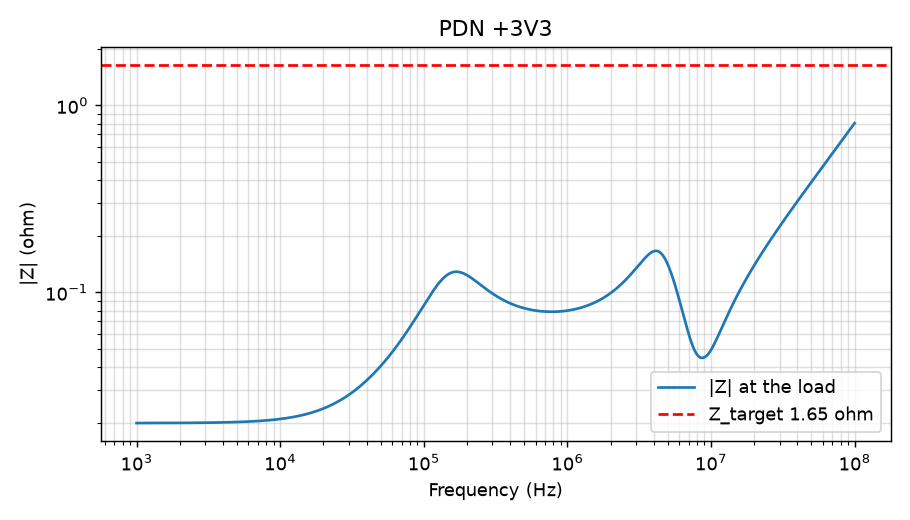
\includegraphics[width=\columnwidth,height=0.45\textheight,keepaspectratio]{../../analysis/pdn/pdn-_3V3.png}
\caption{PDN impedance against Z\_target: pdn-\_3V3}
\label{fig:pdn-pdn-3V3}
\end{figure}
\begin{figure}[!t]
\centering
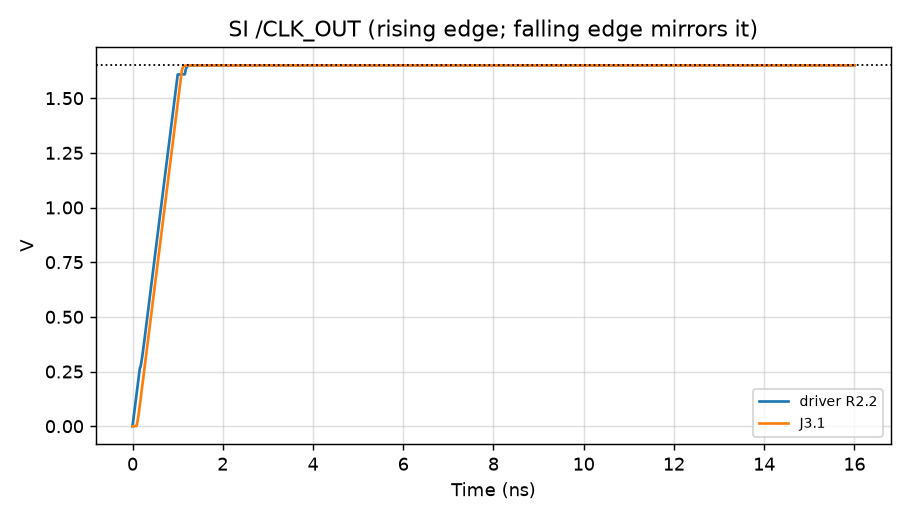
\includegraphics[width=\columnwidth,height=0.45\textheight,keepaspectratio]{../../analysis/si/si-CLK_OUT.png}
\caption{Signal-integrity waveform: si-CLK\_OUT}
\label{fig:si-si-CLK-OUT}
\end{figure}
\begin{figure}[!t]
\centering
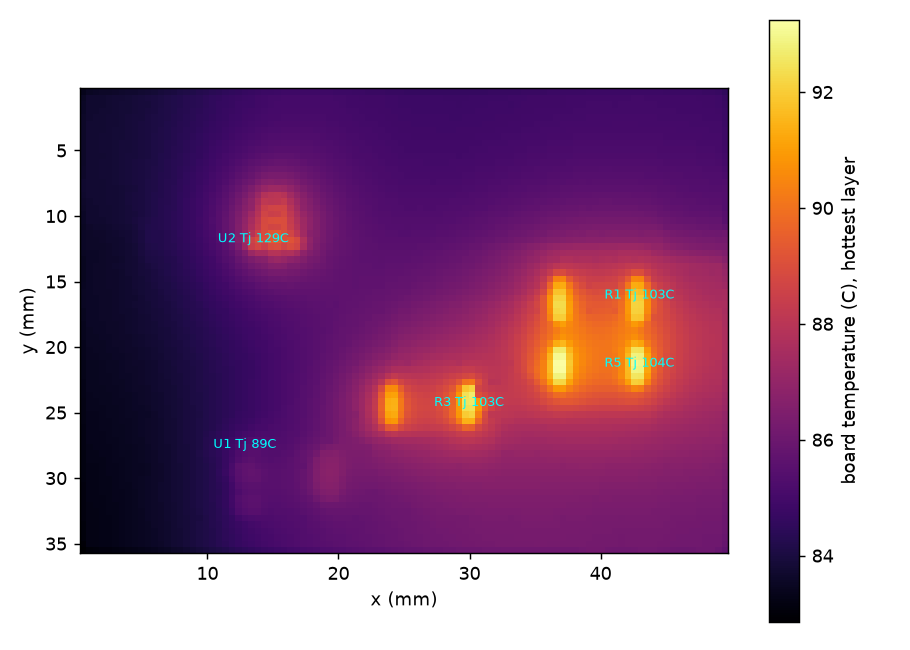
\includegraphics[width=\columnwidth,height=0.45\textheight,keepaspectratio]{../../analysis/thermal/thermal.png}
\caption{Board temperature: thermal}
\label{fig:thermal-thermal}
\end{figure}

\section{Iteration Results}
\begin{table*}[!t]
\caption{Iteration ledger}
\label{tab:iter}
\centering
\scriptsize
\begin{tabularx}{\textwidth}{l|>{\raggedright\arraybackslash}X|l|>{\raggedright\arraybackslash}X|l}
\hline
\textbf{n} & \textbf{change} & \textbf{metric} & \textbf{value} & \textbf{result} \\
\hline
1 & first wired schematic & netlist\_match & MISMATCH (1 label fallback) & discard \\
2 & regenerate after generator fix + fp-lib-table & erc\_violations & 0 & keep \\
3 & first place + Freerouting & drc\_violations & 137-\textgreater{}20 & discard \\
4 & plane fanouts + stitching grid + island removal & drc\_violations & 15 & keep \\
5 & SMA pullback 0.3 mm + scoped edge rule & drc\_violations & 0 & keep \\
6 & denser fence/stitching + launch vias + pre-routed clock & layout\_pass & 53/58-\textgreater{}58/58 & keep \\
7 & bias 2x150R -\textgreater{} 3x220R & rules\_pass & 9/10-\textgreater{}10/10 & keep \\
8 & R1 moved away from U2; 2x3 thermal vias under the GALI tab & tj\_U2 & 130.3-\textgreater{}129.0 C & keep \\
9 & SI deck: merge line fragments shorter than the time step & si\_pass & stall-\textgreater{}4/4 & keep \\
10 & openEMS: capacitors as series ESR-ESL-C, only the analysed and ground nets modelled, band-limited pulse, S-settling row & em\_energy\_db & -11 (never decayed)-\textgreater{}-50 in 28.8k steps & keep \\
11 & In1/In2 cut-out under the SMA centre pads & rf\_in\_S11\_db & -6.8-\textgreater{}-15.9 & keep \\
12 & DC blocks and RF bypass 100 pF -\textgreater{} 10 pF C0G (series-resonant near 2.4 GHz) & R-05\_ohm & 8.8-\textgreater{}3.1 & keep \\
13 & EM launch port driven across the coplanar gaps instead of a 1.5 mm tall vertical sheet to B.Cu & rf\_in\_S11\_db & -14.95-\textgreater{}-17.1 & keep \\
\hline
\end{tabularx}
\end{table*}


\section{Conclusion}
Summarize what was demonstrated, the remaining blockers and the intended next gate.

\bibliographystyle{IEEEtran}
\bibliography{refs}
\end{document}
